\documentclass[11pt, letterpaper, titlepage]{article}
\usepackage[utf8]{inputenc}
\usepackage{geometry}
\usepackage{color,graphicx,overpic} 
\usepackage{fancyhdr}
\usepackage{amsmath,amsthm,amsfonts,amssymb}
\usepackage{mathtools}
\usepackage{hyperref}
\usepackage{multicol}
\usepackage{array}
\usepackage{float}
\usepackage{blindtext}
\usepackage{longtable}
\usepackage{scrextend}
\usepackage[font=small,labelfont=bf,labelformat=empty]{caption}
\usepackage[framemethod=tikz]{mdframed}
\usepackage{calc}
\usepackage{titlesec}
\usepackage{listings}
\usepackage[normalem]{ulem}
\usepackage{tabularx}
\usepackage{mathrsfs}
\usepackage{bookmark}
\usepackage{apple_emoji}
\usepackage{setspace}
\usepackage{ragged2e}
\usepackage{ltablex}
\usepackage{xurl}
\usepackage{siunitx}
\usepackage{lastpage}
\usepackage{enumitem}
\usepackage{minted}
\usepackage{paracol}

\mathtoolsset{showonlyrefs}  
\allowdisplaybreaks

\DeclarePairedDelimiter\ceil{\lceil}{\rceil}
\DeclarePairedDelimiter\floor{\lfloor}{\rfloor}
\DeclarePairedDelimiter\bracks{\left(}{\right)}

\newcolumntype{b}{X}
\newcolumntype{s}{>{\hsize=.5\hsize}X}

\definecolor{bg}{rgb}{0.95,0.95,0.95}

\usemintedstyle{tango}
\setminted{linenos}
\setmintedinline{bgcolor=bg,style=bw}

\tikzset{minimum size=1cm}

\geometry{top=2.54cm, left=2.54cm, right=2.54cm, bottom=2.54cm}
\setlength{\headheight}{20pt}
\setlength{\parskip}{0.5cm}
\setlength{\parindent}{0cm}

\newcommand{\B}{
\includegraphics[height=1.5em, valign=B, raise=-0.2em]{BigB.png}} 

\pagestyle{fancy}
\fancyhf{}
\rhead{\B enjamin Kong | 1573684}
\lhead{\textit{CMPUT 204 Assignment 4 🧀}}
\rfoot{Page \thepage\ of\ \pageref{LastPage}}

\begin{document}
\onehalfspacing

\subsection*{Problem 1.}
\begin{enumerate}[label=\alph*)]
    \item In each iteration, \mintinline{C}{Smallest} recursively calls itself with the first half of the array it was passed and the second half of the array it was passed. As such, the recurrence relation is given by 
    \begin{equation}
        T(n) = 2T(n / 2) + c
    \end{equation}
    where $c$ is some constant. We can now solve this using the master theorem. We have $a = 2$, $b = 2$, and $f(n) = c$. We have that $\log_b(a) = \log_{2}(2) = 1$, so $n^{\log_b(a)} = n$. We see that $f(n) \in O(n^{1 - \epsilon})$ for $\epsilon = 0.5$ (although any $0 < \epsilon < 1$ would work), so case 1 applies. We therefore conclude $T(n) \in \Theta(n)$.

    \item The result of each operation is shown below.
    
    \begin{paracol}{2}
    \begin{figure}[H]
    \centering
    \caption{1. \mintinline{C}{Insert(16)} 🚗}
    \scalebox{0.7}{
    \begin{tikzpicture}[level/.style={sibling distance=45mm/#1}]
        \node[circle,draw]{16};
    \end{tikzpicture}
    }
    \end{figure}

    \switchcolumn

    \begin{figure}[H]
    \centering
    \caption{2. \mintinline{C}{Insert(4)} 🚕}
    \scalebox{0.7}{
    \begin{tikzpicture}[level/.style={sibling distance=45mm/#1}]
        \node[circle,draw]{16}
            child{node[circle,draw]{4}}
            child[missing]{};
    \end{tikzpicture}
    }
    \end{figure}
    \end{paracol}

    \begin{paracol}{2}
    \begin{figure}[H]
    \centering
    \caption{3. \mintinline{C}{Insert(3)} 🚙}
    \scalebox{0.7}{
    \begin{tikzpicture}[level/.style={sibling distance=45mm/#1}]
        \node[circle,draw]{16}
            child{node[circle,draw]{4}
                child{node[circle,draw]{3}}
                child[missing]{}
            }
            child[missing]{};
    \end{tikzpicture}
    }
    \end{figure}
        
    \switchcolumn

    \begin{figure}[H]
    \centering
    \caption{4. \mintinline{C}{Insert(9)} 🚌}
    \scalebox{0.7}{
    \begin{tikzpicture}[level/.style={sibling distance=45mm/#1}]
        \node[circle,draw]{16}
            child{node[circle,draw]{4}
                child{node[circle,draw]{3}}
                child{node[circle,draw]{9}}
            }
            child[missing]{};
    \end{tikzpicture}
    }
    \end{figure}
    \end{paracol}

    \begin{paracol}{2}
    \begin{figure}[H]
    \centering
    \caption{5. \mintinline{C}{Insert(1)} 🚎}
    \scalebox{0.7}{
    \begin{tikzpicture}[level/.style={sibling distance=45mm/#1}]
        \node[circle,draw]{16}
            child{node[circle,draw]{4}
                child{node[circle,draw]{3}
                    child{node[circle,draw]{1}}
                    child[missing]{}
                }
                child{node[circle,draw]{9}}
            }
            child[missing]{};
    \end{tikzpicture}
    }
    \end{figure}
        
    \switchcolumn

    \begin{figure}[H]
    \centering
    \caption{6. \mintinline{C}{Insert(44)} 🚓}
    \scalebox{0.7}{
    \begin{tikzpicture}[level/.style={sibling distance=45mm/#1}]
        \node[circle,draw]{16}
            child{node[circle,draw]{4}
                child{node[circle,draw]{3}
                    child{node[circle,draw]{1}}
                    child[missing]{}
                }
                child{node[circle,draw]{9}}
            }
            child{node[circle,draw]{44}};
    \end{tikzpicture}
    }
    \end{figure}
    \end{paracol}

    \begin{paracol}{2}
    \begin{figure}[H]
    \centering
    \caption{7. \mintinline{C}{Insert(29)} 🚑}
    \scalebox{0.7}{
    \begin{tikzpicture}[level/.style={sibling distance=45mm/#1}]
        \node[circle,draw]{16}
            child{node[circle,draw]{4}
                child{node[circle,draw]{3}
                    child{node[circle,draw]{1}}
                    child[missing]{}
                }
                child{node[circle,draw]{9}}
            }
            child{node[circle,draw]{44}
                child{node[circle,draw]{29}}
                child[missing]{}
            };
    \end{tikzpicture}
    }
    \end{figure}
        
    \switchcolumn

    \begin{figure}[H]
    \centering
    \caption{8. \mintinline{C}{Delete(1)} 🚒}
    \scalebox{0.7}{
    \begin{tikzpicture}[level/.style={sibling distance=45mm/#1}]
        \node[circle,draw]{16}
            child{node[circle,draw]{4}
                child{node[circle,draw]{3}}
                child{node[circle,draw]{9}}
            }
            child{node[circle,draw]{44}
                child{node[circle,draw]{29}}
                child[missing]{}
            };
    \end{tikzpicture}
    }
    \end{figure}
    \end{paracol}

    \begin{paracol}{2}
    \begin{figure}[H]
    \centering
    \caption{9. \mintinline{C}{Delete(4)} 🚐}
    \scalebox{0.7}{
    \begin{tikzpicture}[level/.style={sibling distance=45mm/#1}]
        \node[circle,draw]{16}
            child{node[circle,draw]{3}
                child[missing]{}
                child{node[circle,draw]{9}}
            }
            child{node[circle,draw]{44}
                child{node[circle,draw]{29}}
                child[missing]{}
            };
    \end{tikzpicture}
    }
    \end{figure}
        
    \switchcolumn

    \begin{figure}[H]
    \centering
    \caption{10. \mintinline{C}{Insert(34)} 🚚}
    \scalebox{0.7}{
    \begin{tikzpicture}[level/.style={sibling distance=45mm/#1}]
        \node[circle,draw]{16}
            child{node[circle,draw]{3}
                child[missing]{}
                child{node[circle,draw]{9}}
            }
            child{node[circle,draw]{44}
                child{node[circle,draw]{29}
                    child[missing]{}
                    child{node[circle,draw]{34}}
                }
                child[missing]{}
            };
    \end{tikzpicture}
    }
    \end{figure}
    \end{paracol}

    \item The result of each operation is shown below.
    
    \begin{figure}[H]
    \centering
    \caption{1. Original ✨AVL✨ tree with height 4.}
    \scalebox{0.7}{
    \begin{tikzpicture}[level/.style={sibling distance=70mm/#1}]
        \node[circle,draw]{50}
            child{node[circle,draw]{20}
                child{node[circle,draw]{10}
                    child{node[circle,draw]{5}
                        child{node[circle,draw]{1}}
                        child[missing]{}
                    }
                    child{node[circle,draw]{15}}
                }
                child{node[circle,draw]{35}
                    child[missing]{}
                    child{node[circle,draw]{40}}
                }
            }
            child{node[circle,draw]{80}
                child{node[circle,draw]{65}}
                child{node[circle,draw]{100}
                    child[missing]{}
                    child{node[circle,draw]{110}}
                }
            };
    \end{tikzpicture}
    }
    \end{figure}

    \begin{figure}[H]
    \centering
    \caption{2. \mintinline{C}{Delete(80)}}
    \scalebox{0.7}{
    \begin{tikzpicture}[level/.style={sibling distance=70mm/#1}]
        \node[circle,draw]{50}
            child{node[circle,draw]{20}
                child{node[circle,draw]{10}
                    child{node[circle,draw]{5}
                        child{node[circle,draw]{1}}
                        child[missing]{}
                    }
                    child{node[circle,draw]{15}}
                }
                child{node[circle,draw]{35}
                    child[missing]{}
                    child{node[circle,draw]{40}}
                }
            }
            child{node[circle,draw,red,dashed]{80}
                child{node[circle,draw]{65}}
                child{node[circle,draw]{100}
                    child[missing]{}
                    child{node[circle,draw]{110}}
                }
            };
    \end{tikzpicture}
    }
    \scalebox{0.7}{
    \begin{tikzpicture}[level/.style={sibling distance=70mm/#1}]
        \node[circle,draw]{50}
            child{node[circle,draw]{20}
                child{node[circle,draw]{10}
                    child{node[circle,draw]{5}
                        child{node[circle,draw]{1}}
                        child[missing]{}
                    }
                    child{node[circle,draw]{15}}
                }
                child{node[circle,draw]{35}
                    child[missing]{}
                    child{node[circle,draw]{40}}
                }
            }
            child{node[circle,draw]{65}
                child[missing]{}
                child{node[circle,draw]{100}
                    child[missing]{}
                    child{node[circle,draw]{110}}
                }
            };
    \end{tikzpicture}
    }
    \end{figure}

    \begin{figure}[H]
    \centering
    \caption{3. Single rotate left}
    \scalebox{0.7}{
    \begin{tikzpicture}[level/.style={sibling distance=70mm/#1}]
        \node[circle,draw]{50}
            child{node[circle,draw]{20}
                child{node[circle,draw]{10}
                    child{node[circle,draw]{5}
                        child{node[circle,draw]{1}}
                        child[missing]{}
                    }
                    child{node[circle,draw]{15}}
                }
                child{node[circle,draw]{35}
                    child[missing]{}
                    child{node[circle,draw]{40}}
                }
            }
            child{node[circle,draw]{100}
                child{node[circle,draw]{65}}
                child{node[circle,draw]{110}}
            };
    \end{tikzpicture}
    }
    \end{figure}

    \begin{figure}[H]
    \centering
    \caption{4. Single rotate right}
    \scalebox{0.7}{
    \begin{tikzpicture}[level/.style={sibling distance=70mm/#1}]
        \node[circle,draw]{20}
            child{node[circle,draw]{10}
                child{node[circle,draw]{5}
                    child{node[circle,draw]{1}}
                    child[missing]{}
                }
                child{node[circle,draw]{15}}
            }
            child{node[circle,draw]{50}
                child{node[circle,draw]{35}
                        child[missing]{}
                        child{node[circle,draw]{40}}
                    }
                child{node[circle,draw]{100}
                    child{node[circle,draw]{65}}
                    child{node[circle,draw]{110}}
                }
            };
    \end{tikzpicture}
    }
    \end{figure}

    \item The state of the hash table after each operation is given below.
    \begin{paracol}{2}
        \begin{table}[H]
            \small
            \centering
            \caption{1. \mintinline{C}{Insert(18)} $\rightarrow h(18) = 0$}
            \begin{tabular}{|m{3em}|m{7em}|}
                \hline
                0 & 18 \\ \hline
                1 &  \\ \hline
                2 &  \\ \hline
                3 &  \\ \hline
                4 &  \\ \hline
                5 &  \\ \hline
                6 &  \\ \hline
                7 &  \\ \hline
                8 &  \\ \hline
            \end{tabular}
        \end{table}

        \switchcolumn

        \begin{table}[H]
            \small
            \centering
            \caption{2. \mintinline{C}{Insert(22)} $\rightarrow h(22) = 4$}
            \begin{tabular}{|m{3em}|m{7em}|}
                \hline
                0 & 18 \\ \hline
                1 &  \\ \hline
                2 &  \\ \hline
                3 &  \\ \hline
                4 & 22 \\ \hline
                5 &  \\ \hline
                6 &  \\ \hline
                7 &  \\ \hline
                8 &  \\ \hline
            \end{tabular}
        \end{table}

        \switchcolumn

        \begin{table}[H]
            \small
            \centering
            \caption{3. \mintinline{C}{Insert(32)} $\rightarrow h(32) = 5$}
            \begin{tabular}{|m{3em}|m{7em}|}
                \hline
                0 & 18 \\ \hline
                1 &  \\ \hline
                2 &  \\ \hline
                3 &  \\ \hline
                4 & 22 \\ \hline
                5 & 32 \\ \hline
                6 &  \\ \hline
                7 &  \\ \hline
                8 &  \\ \hline
            \end{tabular}
        \end{table}

        \switchcolumn

        \begin{table}[H]
            \small
            \centering
            \caption{4. \mintinline{C}{Insert(8)} $\rightarrow h(8) = 8$}
            \begin{tabular}{|m{3em}|m{7em}|}
                \hline
                0 & 18 \\ \hline
                1 &  \\ \hline
                2 &  \\ \hline
                3 &  \\ \hline
                4 & 22 \\ \hline
                5 & 32 \\ \hline
                6 &  \\ \hline
                7 &  \\ \hline
                8 & 8 \\ \hline
            \end{tabular}
        \end{table}

        \switchcolumn

        \begin{table}[H]
            \small
            \centering
            \caption{5. \mintinline{C}{Insert(6)} $\rightarrow h(6) = 6$}
            \begin{tabular}{|m{3em}|m{7em}|}
                \hline
                0 & 18 \\ \hline
                1 &  \\ \hline
                2 &  \\ \hline
                3 &  \\ \hline
                4 & 22 \\ \hline
                5 & 32 \\ \hline
                6 & 6 \\ \hline
                7 &  \\ \hline
                8 & 8 \\ \hline
            \end{tabular}
        \end{table}

        \switchcolumn

        \begin{table}[H]
            \small
            \centering
            \caption{6. \mintinline{C}{Insert(10)} $\rightarrow h(10) = 1$}
            \begin{tabular}{|m{3em}|m{7em}|}
                \hline
                0 & 18 \\ \hline
                1 & 10 \\ \hline
                2 &  \\ \hline
                3 &  \\ \hline
                4 & 22 \\ \hline
                5 & 32 \\ \hline
                6 & 6 \\ \hline
                7 &  \\ \hline
                8 & 8 \\ \hline
            \end{tabular}
        \end{table}

        \switchcolumn

        \begin{table}[H]
            \small
            \centering
            \caption{7. \mintinline{C}{Insert(20)} $\rightarrow h(20) = 2$}
            \begin{tabular}{|m{3em}|m{7em}|}
                \hline
                0 & 18 \\ \hline
                1 & 10 \\ \hline
                2 & 20 \\ \hline
                3 &  \\ \hline
                4 & 22 \\ \hline
                5 & 32 \\ \hline
                6 & 6 \\ \hline
                7 &  \\ \hline
                8 & 8 \\ \hline
            \end{tabular}
        \end{table}

        \switchcolumn

        \begin{table}[H]
            \small
            \centering
            \caption{8. \mintinline{C}{Insert(16)} $\rightarrow h(16) = 7$}
            \begin{tabular}{|m{3em}|m{7em}|}
                \hline
                0 & 18 \\ \hline
                1 & 10 \\ \hline
                2 & 20 \\ \hline
                3 &  \\ \hline
                4 & 22 \\ \hline
                5 & 32 \\ \hline
                6 & 6 \\ \hline
                7 & 16 \\ \hline
                8 & 8 \\ \hline
            \end{tabular}
        \end{table}

        \switchcolumn

        \begin{table}[H]
            \small
            \centering
            \caption{9. \mintinline{C}{Insert(2)} $\rightarrow h(2) = 2$}
            \begin{tabular}{|m{3em}|m{7em}|}
                \hline
                0 & 18 \\ \hline
                1 & 10 \\ \hline
                2 & 20 $\leftrightarrow$ 2 \\ \hline
                3 &  \\ \hline
                4 & 22 \\ \hline
                5 & 32 \\ \hline
                6 & 6 \\ \hline
                7 & 16 \\ \hline
                8 & 8 \\ \hline
            \end{tabular}
        \end{table}

        \switchcolumn

        \begin{table}[H]
            \small
            \centering
            \caption{10. \mintinline{C}{Insert(29)} $\rightarrow h(29) = 2$}
            \begin{tabular}{|m{3em}|m{7em}|}
                \hline
                0 & 18 \\ \hline
                1 & 10 \\ \hline
                2 & 20 $\leftrightarrow$ 2 $\leftrightarrow$ 29 \\ \hline
                3 &  \\ \hline
                4 & 22 \\ \hline
                5 & 32 \\ \hline
                6 & 6 \\ \hline
                7 & 16 \\ \hline
                8 & 8 \\ \hline
            \end{tabular}
        \end{table}
    \end{paracol}

    \item Description of algorithm: let $A$ be the final array that will contain all $n$ elements. We first construct a min-heap from the smallest element of each of the $k$ sorted lists. We then extract the first element from the min-heap and add it to $A$. After this, we add the next smallest element from the list from which the extracted element came from. We repeat this process until all elements have been added to $A$.
    
    We now demonstrate this algorithm with an example. Let $L_1 = [2,5]$, $L_2 = [4,8]$, and $L_3 = [3,7]$ be our sorted lists. We first construct a min-heap with the first elements of each of the sorted lists (2, 4, 3) as shown below.
    
    \begin{figure}[H]
    \centering
    \scalebox{0.7}{
    \begin{tikzpicture}[level/.style={sibling distance=35mm/#1}]
        \node[circle,draw]{2}
            child{node[circle,draw]{4}}
            child{node[circle,draw]{3}};
    \end{tikzpicture}
    }
    \end{figure}

    We extract 2 from the min-heap and place it into $A$. At this point, $A = [2]$. Since this element came from $L_1$, we place 5 into the min-heap now.

    \begin{figure}[H]
    \centering
    \scalebox{0.7}{
    \begin{tikzpicture}[level/.style={sibling distance=35mm/#1}]
        \node[circle,draw]{3}
            child{node[circle,draw]{4}}
            child{node[circle,draw]{5}};
    \end{tikzpicture}
    }
    \end{figure}

    We extract 3 from the min-heap and place it into $A$. At this point, $A = [2, 3]$. Since this element came from $L_3$, we place 7 into the min-heap now.

    \begin{figure}[H]
    \centering
    \scalebox{0.7}{
    \begin{tikzpicture}[level/.style={sibling distance=35mm/#1}]
        \node[circle,draw]{4}
            child{node[circle,draw]{5}}
            child{node[circle,draw]{7}};
    \end{tikzpicture}
    }
    \end{figure}

    We extract 4 from the min-heap and place it into $A$. At this point, $A = [2, 3, 4]$. Since this element came from $L_2$, we place 8 into the min-heap now.

    \begin{figure}[H]
    \centering
    \scalebox{0.7}{
    \begin{tikzpicture}[level/.style={sibling distance=35mm/#1}]
        \node[circle,draw]{5}
            child{node[circle,draw]{7}}
            child{node[circle,draw]{8}};
    \end{tikzpicture}
    }
    \end{figure}

    We extract 5 from the min-heap and place it into $A$. At this point, $A = [2, 3, 4, 5]$. This element came from $L_1$, but we have gone through all elements of $L_1$. As such, we do not insert anything into the min-heap.

    \begin{figure}[H]
    \centering
    \scalebox{0.7}{
    \begin{tikzpicture}[level/.style={sibling distance=35mm/#1}]
        \node[circle,draw]{7}
            child{node[circle,draw]{8}}
            child[missing]{};
    \end{tikzpicture}
    }
    \end{figure}

    We extract 7 from the min-heap and place it into $A$. At this point, $A = [2, 3, 4, 5, 7]$. This element came from $L_3$, but we have gone through all elements of $L_3$. As such, we do not insert anything into the min-heap.

    \begin{figure}[H]
    \centering
    \scalebox{0.7}{
    \begin{tikzpicture}[level/.style={sibling distance=35mm/#1}]
        \node[circle,draw]{8};
    \end{tikzpicture}
    }
    \end{figure}

    We finally extract 8 from the min-heap and place it into $A$. We then have $A = [2, 3, 4, 5, 7, 8]$.

    \item \begin{itemize}
        \item Suppose $|R_v| \geq |L_v|$. If we assume $|L_v| = k$, then $|R_v| = 2k$ in the worst case. Since the entire tree contains $n$ nodes, we can say $k + 2k + 1 = n$. This means that $k = (n - 1) / 3$ in the worst case and therefore $|R_v| = 2(n - 1) / 3$. Since only the root needs to be nearly balanced, we can achieve the maximum tree height through a linear distribution of nodes on the right side (basically a linked list after the root). As such, the maximum number of levels is $2(n - 1)/3 + 1$ making the maximum height $2(n - 1)/3$. We conclude that for a tree with 7 nodes, the maximum height is $2(7 - 1)/3 = 4$.
        
        \item As given in problem 7 of problem set \#3, solving the recurrence yields $H_\text{max}(n) = \log_{3/2}((n + 2)/3) + 1$. For $n = 8$, $H_\text{max}(8) \approx 3.97$. Below is an example where we attempt to place as many nodes as possible in the left direction.
        
        \begin{figure}[H]
        \centering
        \scalebox{0.7}{
        \begin{tikzpicture}[level/.style={sibling distance=35mm/#1}]
            \node[circle,draw]{50}
                child{node[circle,draw]{25}
                    child{node[circle,draw]{10}
                        child{node[circle,draw]{1}}    
                        child{node[circle,draw]{12}}    
                    }
                    child{node[circle,draw]{30}}
                }
                child{node[circle,draw]{75}
                    child{node[circle,draw]{60}}
                    child[missing]{}
                };
        \end{tikzpicture}
        }
        \end{figure}

        As we can see, there is no way to move a node such that the height of the tree is greater than 3 while ensuring the tree is nearly balanced. It appears that using the solution to the equation provides an upper bound to the maximum height if we take the floor of the result (i.e. $\floor*{3.97} = 3$).
        
        \item As shown in the previous part, the height of a nearly balanced tree is in $O(\log(n))$. Also, when searching for an element, we know the worst case is when we need to search all the way from the root to the lowest node. Since the height is in $O(\log(n))$, we conclude that the running time for searching for an element is in $O(\log(n))$.
    \end{itemize}

    \item We have 10 bottles of wine 🍷. From problem 9 of problem set \#3, we claim we only need $k = \floor*{\log(n)} + 1 = 4$ testers 😋. Consider the binary representation of 10, $1010_2$, which has $k = 4$ digits. The poisonous bottle 😭 has an unknown index $X$ where $0001_2 \leq X \leq 1010_2$. Tester $i$ tests all bottles of wine whose index (in binary) is 1 at position $i$. If tester $i$ dies after a month 💀, it means that the index of the poisonous bottle in binary has a 1 at position $i$. Otherwise, if the tester survives 😎, it means that the index of the poisonous bottle in binary has a 0 at position $i$. This allows us to determine exactly which bottle of wine is poisoned.
    
    For example, let's say the fifth bottle ($0101_2$) is poisoned. Tester 1 tests bottles 1 ($0001_2$), 3 ($0011_2$), 5 ($0101_2$), 7 ($0111_2$), and 9 ($1001_2$). Since tester 1 dies, we now know the poisoned bottle must contain a 1 at binary position 1. We repeat similar logic for testers 2, 3, and 4 to determine if the poisoned bottle must contain a 1 at binary position 2, 3, and 4 respectively. Eventually, this allows us to conclude the index of the poisoned bottle of wine is $0101_2 = 5$. 
\end{enumerate}

\newpage
\subsection*{Problem 2.}
\begin{enumerate}[label=\alph*)]
    \item For a 3-ary heap implicitly represented by array $A$, given index $i$ we have
    \begin{itemize}
        \item $A[ \floor*{\frac{i - 2}{3} + 1} ]$ is the parent of $A[i]$,
        \item $A[ 3i - 1 ]$ is the left child of $A[i]$,
        \item $A[ 3i ]$ is the middle child of $A[i]$,
        \item $A[ 3i + 1 ]$ is the right child of $A[i]$.
    \end{itemize}

    \item We define the height $h$ as the number of edges on the longest root-to-leaf path. To calculate the height of a 3-ary heap with $n$, elements, we note that the number of nodes at some level $i$ is $3^i$. Let's say that our 3-ary heap contains filled levels from level 0 up to and including level $k$. Then the number of nodes up to and including level $k$ is
    \begin{align}
        \sum_{i = 0}^k 3^i = \dfrac{3^{k + 1} - 1}{3 - 1} = \dfrac{3^{k + 1} - 1}{2}.
    \end{align}
    We now note that the last node, node $n$, either resides in the last filled level (level $k$) or the level after the last filled level (level $k + 1$). Therefore we have the inequality
    \begin{equation}
        \dfrac{3^{k + 1} - 1}{2} \leq n \leq \dfrac{3^{k + 2} - 1}{2}.
    \end{equation}
    Multiplying by 2, adding 1, applying a logarithm with base 3, and subtracting 1 from all expressions yields
    \begin{equation}
        k \leq \log_3(2n + 1) -1 \leq k + 1.
    \end{equation}
    Notice that if the last node, node $n$, is the last node in level $k$, then the last node is $k$ edges away from the root node. Otherwise, the last node is in level $k + 1$ and $\log_3(2n + 1) - 1$ will not be an integer value. As a result, we conclude that applying the ceiling operator to $\log_3(2n + 1) - 1$ will yield the right level. We conclude the height the height of a 3-ary heap of $n$ elements is given by 
    \begin{align}
        h = \ceil*{\log_3(2n + 1) - 1}.
    \end{align}

    \item The code for \mintinline{C}{MaxHeapify} for a 3-ary max-heap is provided below, written in Lua. Note that Lua arrays, unlike arrays in most programming languages, begin indexing at 1.
    \begin{minted}{lua}
function GetLeftChild(i)
    return 3 * i - 1
end

function GetMiddleChild(i)
    return 3 * i
end

function GetRightChild(i)
    return 3 * i + 1
end

function GetHeapSize(A)
    return #A
end

function MaxHeapify(A, i)
    LeftChild = GetLeftChild(i)
    MiddleChild = GetMiddleChild(i)
    RightChild = GetRightChild(i)
    HeapSize = GetHeapSize(A)
    Largest = i
    
    if LeftChild <= HeapSize and A[LeftChild] > A[Largest] then
        Largest = LeftChild
    end
    
    if MiddleChild <= HeapSize and A[MiddleChild] > A[Largest] then
        Largest = MiddleChild
    end
    
    if RightChild <= HeapSize and A[RightChild] > A[Largest] then
        Largest = RightChild
    end
    
    if not (Largest == i) then
        A[i], A[Largest] = A[Largest], A[i]
        MaxHeapify(A, Largest)
    end
end
    \end{minted}
    We can see that the number of times \mintinline{C}{MaxHeapify} calls itself is bounded by the height of the 3-ary heap. From the previous part, we know the height is given by $h = \ceil*{\log_3(2n + 1) - 1}$. We note that the dominant term in the height is $\log_3(2n + 1)$ which is trivially in $O(\log_3(n))$. We also know 
    \begin{equation}
        \log_3(n) = \dfrac{\log(n)}{\log(3)} \in O(\log(n)).
    \end{equation}
    As such, we can conclude that the running time of \mintinline{C}{MaxHeapify} is in $O(\log(n))$. 

    \item The code for \mintinline{C}{BuildMaxHeap} for a 3-ary max-heap is provided below, written in Lua. Note that line 2 is essentially declaring a loop that starts its counter at $\floor*{\text{HeapSize}(A) / 2}$ and decrements down to 1.
    \begin{minted}{lua}
function BuildMaxHeap(A)
    for i = math.floor(GetHeapSize(A) / 2), 1, -1 do
        MaxHeapify(A, i)
    end
end
    \end{minted}
    We can see that \mintinline{C}{BuildMaxHeap} makes about $n/2$ calls to \mintinline{C}{MaxHeapify}. As a result, we can conclude that the running time of \mintinline{C}{BuildMaxHeap} is in $O(n\log(n))$.

    \item After invoking \mintinline{C}{BuildMaxHeap}, we have $A = [12, 10, 6, 4, 7, 2, 8, 5]$. This indeed satisfies the conditions of a 3-ary heap as shown below.
    \begin{figure}[H]
    \centering
    \begin{tikzpicture}[level/.style={sibling distance=55mm/#1/#1}]
        \node[circle,draw]{12}
            child{node[circle,draw]{10}
                child{node[circle,draw]{7}}
                child{node[circle,draw]{2}}
                child{node[circle,draw]{8}}
            }
            child{node[circle,draw]{6}
                child{node[circle,draw]{5}}
                child[missing]{}
                child[missing]{}
            }
            child{node[circle,draw]{4}};
    \end{tikzpicture}
    \end{figure}
    
\end{enumerate}

\newpage
\subsection*{Problem 3.}
The algorithm \mintinline{C}{FindInRange} is given below, written in Lua. Note that Lua arrays begin indexing at 1. \mintinline{C}{FindInRange} is initially called with $i = 1$ (i.e. the root node).
\begin{minted}{lua}
function GetLeftChild(i)
    return 2 * i
end

function GetRightChild(i)
    return 2 * i + 1
end

function GetHeapSize(A)
    return #A
end

function FindInRange(A, i, x, y)
    HeapSize = GetHeapSize(A)
    
    if A[i] < x then
        return
    end
    
    if A[i] <= y then
        print(A[i])
    end
    
    local LeftChild = GetLeftChild(i)
    local RightChild = GetRightChild(i)
    
    if LeftChild <= HeapSize then
        FindInRange(A, LeftChild, x, y)
    end
    
    if RightChild <= HeapSize then
        FindInRange(A, RightChild, x, y)
    end
end
\end{minted}
In the worst case, all elements satisfy $x \leq z \leq y$. In this case, \mintinline{C}{FindInRange} touches each element exactly once and hence the worst case running time is in $O(n)$. We conclude $O(n) \in O(k)$ since $n = k$ in the worst case.

The algorithm is more efficient than a linear search (unless all elements satisfy $x \leq z \leq y$ in which case the efficiency is equal). Notice that if the root of any given subtree is less than $x$, that means all children of that subtree will be less than $x$. This means all the elements in that subtree won't satisfy $x \leq z \leq y$. This knowledge gives us the ability to not search the subtree if its root is less than $x$. This means that in an average case, our algorithm doesn't have to iterate recursively through all elements in the tree making it more efficient than a linear search which must iterate through all elements of $A$ no matter what.

\newpage
\subsection*{Problem 4.}
\begin{itemize}
    \item The worst case occurs when, for each recursive call, the partitions produced during partitioning are of size $n - 1$. When this happens, each recursive call processes a partition that is only one smaller than the previous recursive call. This means we require $n - 1$ recursive calls until we reach a partition of size 1. Since each recursive call $i$ needs to do $n - i$ comparisons against the jars and $n - i - 1$ comparisons against the lids, the running time in the worst case is in $O(n^2)$. 
    
    More formally, the number of key comparisons required by the algorithm is given by the recurrence 
    \begin{equation}
        T(n) = \begin{cases}
            0, & n \leq 1, \\
            T(n_1) + T(n - 1 - n_1) + (2n - 1), & n \geq 2,
        \end{cases}
    \end{equation}
    where $n_1$ is the pivot chosen. Note that $0 \leq n_1 \leq n - 1$. The recurrence is similar to quicksort with the difference that each recursive call needs to do $2n - 1$ comparisons (we compare a lid against $n$ jars and a jar against $n - 1$ lids, so $n + n - 1 = 2n - 1$). 
    
    The worst case occurs when $n_1 = n - 1$. Then we have 
    \begin{equation}
        T(n) = \begin{cases}
            0, & n \leq 1, \\
            T(n - 1) + (2n - 1), & n \geq 2.
        \end{cases}
    \end{equation}
    Expanding out the recurrence, we have 
    \begin{align}
        T(n) &= T(n - 1) + (2n - 1) \\
        &= T(n - 2) + (2n - 3) + (2n - 1) \\
        &= T(n - 3) + (2n - 5) + (2n - 3) + (2n - 1) \\
        &= \ldots \\
        &= T(1) + 3 + 5 + \ldots + (2n - 5) + (2n - 3) + (2n - 1) \\
        &= 3 + 5 + \ldots + (2n - 5) + (2n - 3) + (2n - 1).
    \end{align}
    This is essentially all odd numbers up to $2n - 1$ except for 1. So we have
    \begin{align}
        T(n) &= \sum_{i = 1}^n (2i - 1) - 1 \\
        &= n^2 - 1.
    \end{align}
    So, $T(n) \in \Theta(n^2)$ in the worst case.

    \item We have $n = 7$. We assume our algorithm solves all subproblems correctly (i.e. our algorithm holds for any array with size $<7$). 
    
    We first take the last lid $l_4$ as the pivot. We then compare this lid against all $n$ jars. We are able to match $l_4$ with $j_4$. Furthermore, all jars smaller than $l_4$ are placed to the left of $j_4$ (let us denote this set by $J_s$) and all jars larger than $l_4$ are placed to the right of $j_4$ (let us denote this set by $J_l$). 
    
    We then use jar $j_4$ to compare against all lids (except $l_4$). This allows us to partition all lids smaller than $j_4$ to the left of $l_4$ (let us denote this set by $L_s$) and all lids larger than $j_4$ to the right of $l_4$ (let us denote this set by $L_l$). 
    
    We now apply our algorithm to each new jar and lid pair, i.e., we use our algorithm on $J_s$ and $L_s$, then on $J_l$ and $L_l$. Each of these sets contain $n = 3$ elements, so based on our assumption, our algorithm will match all jars to their corresponding lids.

    \item As described in the previous part, the worst case running time is in $O(n^2)$. This scenario is guaranteed to happen if the lids are in sorted order from smallest to largest: for each recursive call, the lid selected is the largest in the partition, so all other lids are placed in partition $L_s$.
    
    The best case occurs when, for each recursive call, the partitions produced during partitioning are approximately of size $n / 2$. When this happens, each recursive call produces a partition that is about half the size of the previous recursive call. This means we require approximately $\log(n)$ recursive calls until we reach a partition of size 1. Since each recursive call $i$ needs to do $n - i$ comparisons, the running time in the best case is in $O(n\log(n))$.
\end{itemize}

\end{document}
